\documentclass[12pt,titlepage,french]{article}
\usepackage{babel}
\usepackage{graphicx}
\usepackage[margin=2.5cm]{geometry}

\usepackage[hidelinks]{hyperref}
\usepackage{tabularx}
\usepackage[utf8]{inputenc}
\usepackage[T1]{fontenc}
\pagestyle{plain}

\usepackage{booktabs,makecell,tabu}
\renewcommand\theadfont{\bfseries}

\linespread{1.5}

\newcounter{firstbib}

\begin{document}
%\renewcommand{\thesection}{\arabic{section}} % utilisé pour spécifier la numérotation des sections

\begin{titlepage}
\newcommand{\HRule}{\rule{\linewidth}{0.5mm}}
\center

  
\includegraphics[width=0.45\textwidth]{../../ressources/img_logos/logo_polytech.png}\\[1cm]

  
\includegraphics[width=0.45\textwidth]{../../ressources/img_logos/logo_taglabs.png}


\HRule \\[0.4cm]
{ \huge \bfseries Rapport itération 1\\[0.15cm] }
Classification colorimétrique de nuages de points 3D\\
Version 1.1\\
Le \today \\
\HRule \\[1.5cm]
Ronan Collier,
Mathieu Letrone,
Tri-Thien Truong
\\[1cm]
\end{titlepage}

\tableofcontents % table des matières
\newpage
\listoffigures  % table des figures
\newpage

\section{Remerciements}

Avant de commencer la présentation de notre première itération sur notre projet transversal, nous voulions, une nouvelle fois, remercier notre client M. Yan Koch, et M. Nicolas Normand, pour leur investissement et de leur présence aux réunions.

De plus, nous remercions M. Aurelien Milliart, qui a rejoint M. Yan Koch, pour avoir participé à nos réunions, qui s'intéresse et offre son aide pour que nous puissions mener à bien ce projet.

\section{Rappel des objectifs de l'itération}
La présente itération avait pour objectif principal l'étude des techniques qui vont être utilisées pour les itérations suivantes.
Il s'agit d'un travail principalement de recherche, et de documentation. En effet, nous voulons être sûr du langage à utiliser, et des bibliothèques qui nous seront utiles pour le projet, avant de commencer à développer notre première solution.

Les principales tâches à réaliser durant cette première itération sont les suivantes :
\begin{itemize}
  \item Se renseigner sur l'implémentation d'un plugin pour CloudCompare
  \item Recherches de bibliothèques liées aux traitements de nuages de points (pour les langages C++, et/ou Python)
  \item Recherches sur le langage qui serait le plus intéressant à utiliser pour notre projet
  \item Commencer à réfléchir sur l'organisation, l'architecture du code source
  \item Trouver et comparer des espaces colorimétriques pour un nuage de points
  \item Rechercher des algorithmes de segmentation, à des méthodes pour isoler des points/éléments dans le nuage
  \item Rechercher des méthodes pour réaliser de la fausse couleur dans le nuage
\end{itemize}

L'ensemble de ces tâches vont nous permettre à la fin de l'itération, de partager nos recherches avec notre tuteur académique et notre client, et de choisir les outils les plus adaptés pour la production de notre projet.

\section{Production / réalisation durant l'itération}

\subsection{Interrogation du plugin pour CloudCompare}

La réalisation d'un plugin CloudCompare avait à être explorée. Le fait d'utiliser CloudCompare comme logiciel de fondement pour le projet, aurait pu nous permettre la gestion de la lecture, manipulation et visualisation des nuages de points via celui-ci. Cela, nous permettrait de nous concentrer sur l'algorithmie et l'implémentation de la segmentation et de la fausse couleur.
Le logiciel est sous licence "GNU General Public License", ce qui vise à garantir des droits à l'utilisateur.
\begin{itemize}
\item Liberté 0. La liberté d'exécuter le logiciel, pour n'importe quel usage ;
\item Liberté 1. La liberté d'étudier le fonctionnement d'un programme et de l'adapter à ses besoins, ce qui passe par l'accès aux codes sources ;
\item Liberté 2. La liberté de redistribuer des copies ;
\item Liberté 3. L'obligation de faire bénéficier la communauté des versions modifiées
\end{itemize}

Ainsi, suivant ces libertés, nous sommes autorisés de modifier le programme en ajoutant ledit plugin et nous ne sommes pas tenus de le publier tant qu'il s'agit d'un usage local. Dans le cas d'une distribution, il faudrait le distribuer sous la même licence.

Le Git de CloudCompare est prévu pour accueillir des contributions au logiciel, cependant, la documentation sur la manœuvre à suivre se focalise sur les normes syntaxiques à respecter plutôt que sur la marche à suivre pour créer le plugin.
Malgré la faisabilité de la chose, on peut se demander s'il est vraiment nécessaire d'y avoir recours, tout en sachant que des bibliothèques Python et C++ permettent une lecture et manipulation de nuages de points.\\
Suite au sprint review, nous nous sommes accordés sur le fait de diriger le projet sur la conception d'un plugin CloudCompare. Cela pourra être une bonne expérience d'interagir avec un logiciel très connu dans le monde du nuage de points 3D.

\subsection{Bibliothèques liées aux traitements de nuages de points}

Nous avons produit un comparatif des bibliothèques C++ et Python permettant la manipulation de nuage de points et la segmentation.
Nous avons également développé des scripts Python courts permettant de nous familiariser avec les nuages de points, et de tester les différentes bibliothèques.

Après nos recherches sur les bibliothèques, celles que nous avons relevé liées aux nuages de points, sont utilisables en C++ et Python.

Un tableau récapitulatif sur ces bibliothèques est le suivant : \\

\noindent\begin{tabu} to \textwidth {X[l]X[l]}\toprule
  \thead{Bibliothèques dans les 2 langages}&\thead{Remarques pour le projet}\\\toprule
PCL : Beaucoup de fonctionnalités. Mais utiliser PCL nécessite d’utiliser des fichiers d’entrée de format \og.pcd\fg (Point Cloud Data). Licence BSD (libre).
& Pour avoir essayé cette bibliothèque, il est assez facile de l’utiliser et de charger le nuage de points en entrée dans un objet.\\\midrule
PDAL (format LAS, pour du traitement de nuages de points lidar (light detection and radar))
& Le format LAS est très utilisé pour les données en 3D. Le problème est que ce format de fichier est très volumineux, car il contient de nombreuses informations pour chaque point (x,y,z,i,numéro de retour, angle de balayage…).

Par rapport à la bibliothèque, il y a moins de documentation par rapport à PCL.
\\\midrule
CGAL => bibliothèque pour des calculs géométriques (2D/3D).
& Elle fournit de nombreux algorithmes, similaires à PCL.\\\midrule
Opend3D => Permet de traiter des données 3D.
&  Ici, cette bibliothèque traite la 3D en général, et n’est pas spécialisé dans les nuages de points 3D.\\\bottomrule \\
\end{tabu}

Pour conclure sur cette partie, PCL pourrait être la bibliothèque qui nous servira le plus dans le contexte de notre projet, de part sa facilité à utiliser, et des fonctionnalités qu'elle peut nous apporter pour développer nos algorithmes.

Nous avions tout de même quelques questions par rapport aux formats que le client pourrait nous fournir. En effet, pour l'instant, nous avions des nuages de points en format texte. Il nous fallait alors réfléchir à un moyen pour traiter ces données. Grâce à CloudCompare, il est possible de charger le nuage de points en format texte (ou autre) sur le logiciel, puis de l'exporter au format que nous voulons (ici, au format PCD).

\subsection{Langage : C++, Python, ou autres ?}

Pour cette partie, nous pensions au départ qu'il allait y avoir des différences au niveau des outils qui pourraient être propre au C++ ou au Python. Comme dit précédemment, nous avons remarqué au final, que les bibliothèques étaient utilisables dans les deux langages. Le comparatif s'est alors surtout posé sur les langages en eux-mêmes.

Nous avons réalisé un tableau comparatif entre ces langages : \\

\noindent\begin{tabu} to \textwidth {X[c]X[c]}\toprule
  \thead{C++}&\thead{Python}\\\toprule
+ Langage compilé
& + Langage interprété\\\midrule
+ Rapidité
& - Plus lent que le C++\\\midrule
+ Langage bas niveau
& + Langage plus haut niveau\\\midrule
+ Compatible avec CloudCompare
& - Pas compatible avec CloudCompare\\\midrule
- Langage qui peut être complexe à utiliser, adapté pour des systèmes embarqués, des gros programmes
& + Plus simple à prendre en main, permet donc de se focaliser sur les algos\\\midrule
 Bibliothèque ROOT (Panda pour du c++)
& + Bibliothèque Panda (traitement de données, ici pour traiter les fichiers d'entrée en .txt)\\\bottomrule  \\
\end{tabu}

Les majeurs critères sont donc la rapidité, la compatibilité avec CloudCompare (si l'option du plugin est intéressant dans le cadre de notre projet) et la complexité du langage à prendre en main.

Après réunion, comme nous allons nous diriger vers la solution d'un plugin pour CloudCompare, le choix de C++ semble plus intéressant. Toutefois, il serait aussi possible de faire le lien avec CloudCompare en C++, et de faire nos algorithmes en Python dans un premier temps. Après réflexion de notre part, nous avons décidé de réaliser entièrement le projet en C++, et ainsi éviter de faire des dépendances uniquement pour faire nos algorithmes en Python.

\subsection{Architecture du code source}

Nous avons dédié du temps pour réfléchir sur l'architecture du projet. En effet, cela nous permettra de commencer avec un code organisé, et d'éviter de faire du refactoring en milieu de développement. Il nous a été quand même difficile de vraiment imaginer l'organisation du code, puisque le sujet de notre projet porte surtout sur l'implémentation d'algorithmes. Il n'y a donc pas vraiment d'architecture comme un client/serveur, ou autre.

Nous avons tout de même pensé au fait qu'il nous faudra séparer le code qui pourra potentiellement évoluer, avec du code qui sera "fixe". Par exemple, le code fixe sera par exemple des fonctions qui utiliseront les bibliothèques, et d'autres part, les algorithmes que nous développerons.

Ensuite, il nous sera aussi possible de distinguer en plusieurs packages (ensemble de fichiers de code), le code qui servira au pré-traitement des données d'entrée, le code pour la segmentation/isolation d'éléments, et le code pour la sortie (l'exportation).

Après réunion, l'architecture du projet va donc plutôt séparer le code permettant de faire le plugin CloudCompare, et nos algorithmes.

\subsection{Les espaces colorimétriques pour un nuage de points}

Durant ce sprint, nous avons recherché l'espace colorimétrique le plus adéquat pour travailler.
En effet, la segmentation est basée sur la couleur des éléments, ainsi l'espace de couleur est important.
Les principaux espaces sont le RGB, L*a*b* et le CIE XYZ ou encore le HSV.
\begin{itemize}
    \item Le RGB, définit une couleur suivant une proportion de rouge, vert et bleu, cet espace est également la représentation standard des couleurs des points des nuages.
    \item Le HSV, Teinte Saturation Valeur (Hue Saturation Value), n'a pas été retenu, car il n'est pas vraiment un espace de couleur et est basé sur le RGB, mais permet une meilleure représentation/modélisation des couleurs.
IL reste intéressant pour les outils graphiques comme le color picker.
    \item Le CIELab, définit comme le RGB une couleur via une représentation en 3 dimensions. l* : la luminance, a* et b* la chrominance.
\end{itemize}
Cette distinction est particulièrement intéressante. En effet, dans le cas du RGB, les composantes de la couleur d'un object sont toutes corrélées à la proportion de lumière qui l'a frappée, ce qui rends difficile la description suivant ces composantes.

Or, pour le cas de lab, seule la luminance sera impactée. C'est pourquoi, nous pourrions peut-être seulement prendre en compte la chrominance pour la segmentation, cela pourrait palier les différences d'éclairage imputés par les stations.

De plus, le lab plutôt que le CIE XYZ, car bien qu'il soit basé en parti sur le XYZ, il a une plus grande uniformité perceptuelle. Le critère d'uniformité concerne la tolérance pour dire qu'un jeu de couleurs sont acceptablement proche ou non suivant un seuil.

Dans le cas d'une uniformité, le seuil n'est qu'une constante au lieu d'être une fonction.

Cependant, l'utilisation de lab a des désavantages, il faudra réaliser la conversion de RGB à XYZ puis de XYZ à lab avant de pouvoir réaliser le processus de segmentation, et la représentation lab requière plus d'espace mémoire, ce qui est à prendre en compte.

\subsection{Algorithmes de segmentation}
Plusieurs méthodes de segmentations existent. La plus naïve consiste à filtrer les points selon une couleur avec un seuil d'erreur.
Des recherches montrent une méthode alternative plus poussées.
La piste envisageable repose sur 3 étapes.
Premièrement, la classification des points par une méthode basée sur les KNN appliquée à la distance colorimétrique entre les points (Region growing):
$
CD(C_1,C_2)=\sqrt[]{(R_1-R_2)^2 + (G_1-G_2)^2 + (B_1-B_2)^2}
$
Ensuite, on réalise une seconde classification sur les régions afin d'obtenir des groupes de régions homogènes.
Ces groupes sont ensuite fusionnés. La liste des régions de couleurs similaires est alors obtenue.
Une troisième étape dite de raffinement peut être ajoutée. Elle consiste à imposer un seuil minimal de points par régions.
Si une région ne remplit pas cette contrainte, elle est fusionnée avec l'autre région ayant la distance colorimétrique la plus proche.

\subsection{Méthodes pour la fausse couleur}
Dans le cas d'un nuage de points en nuances de gris, ce procédé consiste à faire correspondre la valeur en intensité d'un point avec une couleur en RGB (Rouge, Vert, Bleu), ou d'un autre espace de couleurs.
Les intensités sont découpées en plage de valeurs et chaque plage se voit assigner une couleur RGB, on obtient ainsi une palette de couleurs. L'intensité de chaque point est ensuite remplacée par la couleur associée dans la palette.
Dans l'exemple suivant, on découpe l'échelle d'intensité en 4. Chaque portion se voit attribuer une couleur, que l'on retrouve ensuite sur l'image.

\begin{figure}[!hbtp]
  \caption{\label{} Echelle de fausse couleur et résultat}
  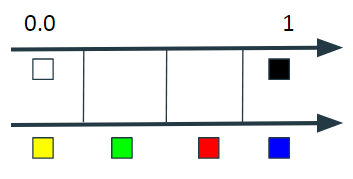
\includegraphics[width=0.45\textwidth]{./img/false_color_scale.png}
  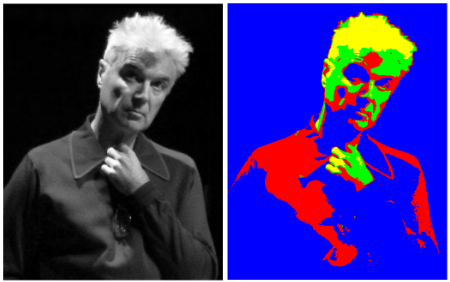
\includegraphics[width=0.45\textwidth]{./img/false_color.png}
\end{figure}
\section{Risques éliminés durant l'itération}
L'itération n'a pas permis l'élimination de risques. En effet, nos risques portent surtout sur la production de nos algorithmes, et des données qui nous sont fournies en entrée. Pour cette itération, nous étions focalisés sur la réalisation de tests sur les différents outils.

\section{Commentaires sur l'itération}

\subsection{Commentaires sur l'itération de façon générale}
L'organisation de l'itération a été difficile étant donné la présence de nombreux examens et des rendus de projets dans les semaines. Toutefois, nous avons pu réaliser l'ensemble de nos tâches prévues pour cette itération.\\
Il nous a été difficile de vraiment montrer quelque chose de concret, puisque nous avons principalement fait de la recherche. La prochaine itération portera davantage sur du développement, et nous pourrons ainsi discuter sur ce que nous aurons produit.

\subsection{Commentaires sur les méthodes de travail/changements de méthode}
Nous avons essayé au maximum de nous répartir sur les tâches à réaliser. Cela nous a permis d'être plus ou moins indépendants sur nos recherches. Néanmoins, nous avons fait, à certains moments, des recherches similaires puisque certaines sources permettaient d'avoir des informations sur les autres recherches à effectuer.

\section{Trois principaux risques restants}
Cette partie est un rappel des principaux risques qu'il faudra garder en mémoire pour les prochaines itérations.

\begin{itemize}
  \item Incapacité à distinguer les éléments de façon efficace dus à des artefacts ou manques d'informations sur une zone du nuage de points
  \item Impact trop important du mouchetage sur la qualité de la segmentation.
  \item Des points résiduels qui restent dans le nuage de points après filtrage (notamment à cause des artefacts).
\end{itemize}

\section{Objectifs de la prochaine itération}
Grâce à cette itération, nous avons effacé des parties floues concernant le projet. En effet, nous avons plus d'informations sur la vision générale du projet et des outils que nous utiliserons. Pour la prochaine itération, les tâches prévues étaient :
\begin{itemize}
  \item Plugin CloudCompare OU lecture / export
  \item Développer la sélection de points selon une couleur définie (via RGB, et/ou LAB)
  \item Développer une solution pour extraire des points dans le nuage.
  \item Mettre le code en commun.
\end{itemize}

Après concertation avec notre client, nous allons donc avoir une tâche pour faire le plugin CloudCompare, et nous n'aurons donc pas à faire la lecture / exportation du nuage de points, puisque ces tâches seront disponibles directement sur l'outil.

\begin{figure}[!hbtp]
  \caption{\label{} Diagramme de Gantt détaillé - Sprint 2}
  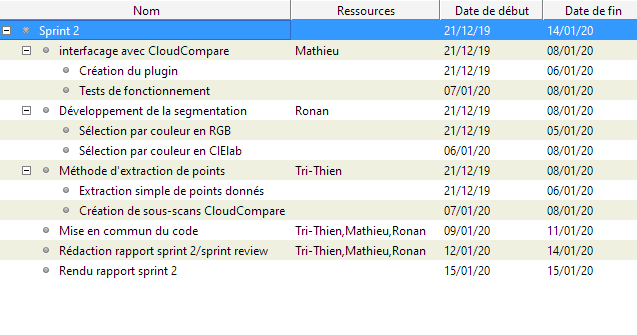
\includegraphics[width=1\textwidth]{./img/sprint_iteration_2_tableau.PNG}
  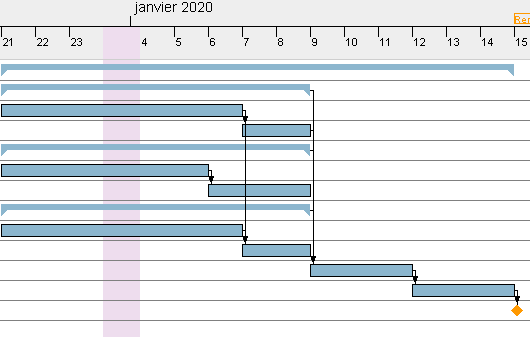
\includegraphics[width=0.8\textwidth]{./img/sprint_iteration_2_diagramme.PNG}
\end{figure}

Ce diagramme présente la deuxième sprint sur le prochain mois à venir. Chacun aura une tâche précise à développer. Une phase entre la période de Noël et le nouvel an est prise en compte dans notre sprint, où nous ne passerons pas forcément du temps sur le projet. 

\section{Résumé}
\subsection{Tâches principales réalisées dans l'itération}
\noindent\begin{tabu} to \textwidth {p{0.18\textwidth}X[c2]X[c]X[c4]}\toprule
  \thead{Tâche}&\thead{Responsable}&\thead{Statut}&\thead{Commentaire}\\\toprule
Plugin pour CloudCompare
& Mathieu
& Achevé
& Plugin CloudCompare possible, ou développer une interface à la main. Le choix est de faire un plugin CloudCompare.\\\midrule
Bibliothèques pour le traitement de nuages de points
& Ronan, Tri-Thien
& Achevé
& PCL semble la bibliothèque principale à utiliser, par sa simplicité et toutes les fonctionnalités qu'elle peut nous fournir.\\\midrule
Choix du langage
& Tri-Thien
& Achevé
& C++ ou Python. Le choix est le C++ pour faciliter l'implémentation du code avec CloudCompare. \\\midrule
Architecture du code source
& Ronan, Tri-Thien, Mathieu
& Achevé
& Organisation avec un package pour le plugin CloudCompare, et un autre pour nos algorithmes.\\\midrule
Espaces colorimétriques
& Mathieu
& Achevé
& Le format RGB est le plus répendu, mais l'option du CIELab semble être intéressant.\\\midrule
Algorithmes de segmentation
& Ronan, Tri-Thien, Mathieu
& Achevé
& Méthode pour segmenter selon une couleur (et un seuil d'erreur). Autre alternative : classification des points et régions puis raffinement\\\midrule
Recherche sur les méthodes de fausses couleurs
& Ronan
& Achevé
& Correspondre une valeur en intensité en RGB (ou autre). Création d'une palette de couleurs.\\\bottomrule  \\
\end{tabu}

\subsection{Tâches principales à réaliser pour la prochaine itération}
\begin{itemize}
  \item Plugin CloudCompare
  \item Développer la sélection de points selon une couleur définie
  \item Développer une solution pour extraire des points dans le nuage
  \item Mettre le code en commun.
\end{itemize}

\newpage

\section {Références}

\renewcommand{\refname}{Segmentation}
\begin{thebibliography}{3}
\bibitem{B01} Qingming Zhan, Yubin Liang, Yinghui Xiao, \textit{Color-based segmentation of point clouds}, 2009

\setcounter{firstbib}{\value{enumiv}}
\end{thebibliography}

\renewcommand{\refname}{Fausse couleur}
\begin{thebibliography}{3}
\setcounter{enumiv}{\value{firstbib}}


\bibitem{B02} Méthode de la fausse couleur sur une image:
\url{https://www.imageeprocessing.com/2016/03/gray-scale-to-pseudo-color.html}

\bibitem{B03} Fausse couleur appliquée à une image en python:
\url{https://stackoverflow.com/questions/31507479/how-to-turn-grayscale-into-false-color-using-pil}

\setcounter{firstbib}{\value{enumiv}}
\end{thebibliography}


\renewcommand{\refname}{C++}
\begin{thebibliography}{3}
\setcounter{enumiv}{\value{firstbib}}

\bibitem{B04} Segmentation de nuages de points 3D pour le phenotypage de tournesols :
\url{https://orasis2017.sciencesconf.org/135580/document?fbclid=IwAR2mng-m55ouiJ3_bqHQE61-_VoJ6M1lQLRzWHLLBfLbt1fZm4StWtCyglY}

\bibitem{B05} Extraction d'éléments géométriques dans un nuage de points LiDAR terrestre : application aux relevés de façades :
\url{https://dumas.ccsd.cnrs.fr/dumas-01164570/document?fbclid=IwAR2jKbrR7yHmLxiV2_BJ0qt5q3Ik-EMz2C5_gcR-mldgtvuCIimlbPOoCDg}

\bibitem{B06} Exemple de chargement d'un fichier de nuage de points :
\url{https://stackoverflow.com/questions/43521711/why-is-the-point-cloud-librarys-loadpcdfile-so-slow}

\bibitem{B07} Lecture d'un fichier .pcd en C++ :
\url{http://pointclouds.org/documentation/tutorials/reading_pcd.php}

\bibitem{B08} Récupérer le R, G et B avec PCL :
\url{http://www.pcl-users.org/Unreadable-RGB-values-almost-everywhere-in-Point-Cloud-td4045585.html}

\setcounter{firstbib}{\value{enumiv}}
\end{thebibliography}


\renewcommand{\refname}{Comparaison C++/Python}
\begin{thebibliography}{3}
\setcounter{enumiv}{\value{firstbib}}

\bibitem{B09} C++ vs Python :
\url{https://www.quora.com/Which-is-better-Python-or-C++}

\bibitem{B10} C++ vs Python :
\url{https://www.bitdegree.org/tutorials/python-vs-c-plus-plus/}

\setcounter{firstbib}{\value{enumiv}}
\end{thebibliography}


\renewcommand{\refname}{Formats de fichier}
\begin{thebibliography}{3}
\setcounter{enumiv}{\value{firstbib}}

\bibitem{B11} Format PCD :
\url{http://pointclouds.org/documentation/tutorials/pcd_file_format.php}

\bibitem{B12} Format LAS :
\url{https://www.onyxscan-lidar.com/le-format-de-fichier-las/ }

\setcounter{firstbib}{\value{enumiv}}
\end{thebibliography}

\renewcommand{\refname}{Espaces colorimétriques}
\begin{thebibliography}{3}
\setcounter{enumiv}{\value{firstbib}}

\bibitem{B13} Leow Wee Kheng, National University of Singapore, \textit{Color Spaces and Color-Difference Equation}
\url{https://www.comp.nus.edu.sg/~leowwk/papers/colordiff.pdf}

\bibitem{B14} Liste non exhautive des espaces de couleur.
\url{https://en.wikipedia.org/wiki/List_of_color_spaces_and_their_uses}

\bibitem{B15} Liste non exhautive des espaces de couleur.
\url{https://en.wikipedia.org/wiki/List_of_color_spaces_and_their_uses}

\bibitem{B16} Comparatif des espaces colorimétrique
\url{https://www.researchgate.net/publication/316961754_Color_Image_Segmentation_using_FCM_Clustering_Technique_in_RGB_Lab_HSV_YIQ_Color_spaces}

\bibitem{B17}CIELAB
\url{https://en.wikipedia.org/wiki/CIELAB_color_space}

\setcounter{firstbib}{\value{enumiv}}
\end{thebibliography}


\end{document}
